\input{plos_header.tex}

\begin{document}

% Title must be 150 characters or less
\begin{flushleft}
{\Large
\textbf{A minimal language for functional closure and the origin of evolvability}
}
% Insert Author names, affiliations and corresponding author email.
\\
Author1$^{1}$, 
Author2$^{2}$, 
Author3$^{3,\ast}$
\\
\bf{1} Author1 Dept/Program/Center, Institution Name, City, State, Country
\\
\bf{2} Author2 Dept/Program/Center, Institution Name, City, State, Country
\\
\bf{3} Author3 Dept/Program/Center, Institution Name, City, State, Country
\\
$\ast$ E-mail: Corresponding author@institute.edu
\end{flushleft}

\listoftodos

% Please keep the abstract between 250 and 300 words
\section*{Abstract}

% Please keep the Author Summary between 150 and 200 words
% Use first person. PLoS ONE authors please skip this step. 
% Author Summary not valid for PLoS ONE submissions.   
\section*{Author Summary}

%%erase/comment out this section once some real comments are present
%\begin{comment}
\section*{Example usage of todo notes}
This is a sentence about which a comment is made in the margin\todo[fancyline, size=\small, color=green!40]{This is an example usage of a todonote todo note.}\todo[color=blue!40]{Todonote with a different color and having the standard thin line back to the same point in the text as the previous note.}. This is an example of a placeholder for a figure:
\missingfigure{insert figure of ...}
\todo[inline, color=red!50]{You can also have inline todonotes.}
This is a paragraph about which a comment is made with no line pointing back into the text\todo[noline]{A note with no line back to the text.}.
%\end{comment}

\section*{Introduction}
%!TEX root = ../notes.tex
The capacities have been demonstrated to chemically synthesize and transplant genomes to alter organismal identity \cite{Gibson2010} and to execute simulations of the life cycle of a single-celled organism \cite{Karr2012} by collecting measurements of a large number of parameter values conveying detailed information about its underlying processes and integrating them into presumably analogous coupled algorithmic processes. These capacities and the technologies that may result from them add to the mounting pressure underlying the very existence of the field of systems biology to ask, in an effort to synthesize knowledge from an enormous number of empirical investigations, whether or not we can abstract properties that are necessary, and perhaps sufficient, for determining a process capable of generating organisms \emph{de novo}. Answering questions like this one are crucial for clarifying hypotheses germane to understanding what is required in order to explain the origin and distinguishing characteristics of life and thus the origin and nature of evolutionary processes.

Very few biologists or other scientists dispute that evolution is the most fundamental organizing concept in biology. In this light, it seems somewhat surprising that not even more effort than has already been exerted is invested in clarifying and formalizing increasingly detailed conceptions of its origins and operation. In order to understand biological systems, it will be necessary to address the question: What are the necessary enabling conditions that make biological evolution possible? The synthesis of some potential answers to this question may clarify a path toward defining a sufficient collection of preconditions for evolutionary processes to take flight.

Here we argue that one such necessary precondition for evolutionary processes, which has been identified before as a ``defining characteristic of life''\cite{Rosen1972,Rosen1978,Rosen1985,Rosen1991}, is what we refer to as \emph{functional closure}. In order to define this term and its context, we begin with a diagrammatic model of a prototypical biochemical reaction network that has been claimed to possess this property. We then ask: Is there a formal language capable of expressing this property? A brief detour is necessary to motivate this question. In computer science, there is a property of languages called \emph{expressive power} that is used both heuristically and formally to rank order models of computation, programming languages, and their associated logics with respect to one another and with respect to so-called \emph{natural language}. Roughly speaking, an increased level of expressive power of a language correlates with its ability to express more complex or sophisticated ideas. One might ask why it is not always desirable to work within the extant language containing the highest possible expressive power. One reason to consider less expressive languages at all is that important questions about them can be answered algorithmically with appropriate computer hardware and software in a practical amount of time and memory, whereas the same questions posed of languages with more expressive power are known not to be able to be answered by such means\cite{Hopcroft2007}. Thus, identifying a \emph{minimal} language capable of expressing the necessary conditions for the origin of evolutionary processes is directly germane to the continuing development of exquisitely detailed models of whole cells as they are refined, unfold and are embedded into equally detailed multi-level models of populations, communities, and ecosystems.

In this light, we can refine the question, ``Is there a formal language capable of expressing the functional closure property?'' by adjoining the follow-up question, ``If so, among those that are, which is the language of minimal expressive power?'' We begin to address the first question taking an historically motivated approach \cite{Rosen1972,Letelier2006} by attempting to interpret the aforementioned diagram expressing functional closure in terms of an abstract algebraic language (category theory). Unfortunately, the prototypical diagram violates a fundamental assumption of this language precisely because the diagram expresses the functional closure property. This diagram, and indeed the functional closure property in general, can be interpreted in terms of a standard model of computation called (untyped or type-free) lambda calculus \cite{Mossio2009}. Via this conceptual route, we find that the interpretation of functional closure in terms of category theory can be recovered, albeit it in a form that looks quite different, via one typical category theoretic semantics for the untyped lambda calculus \cite{Scott1980,Barendregt1985,Abramsky1995}.

Although the untyped lambda calculus and its associated category theoretic semantics are capable of expressing the functional closure property, this method has at least two problems. One is that the untyped lambda calculus is a, relatively speaking, highly expressive language capable of implementing general recursion. The second is that the untyped lambda calculus is capable of expressing functional closure in a trivial way via something as simple as an identity function. A simple solution might seem to pass to the simply typed lambda calculus, of which the untyped lambda calculus has been argued to be a special case. However, as a result of the analogous category theoretic semantics for the simply typed lambda calculus, doing so brings us back to the original category theoretic interpretation of the diagram expressing the functional closure property that we demonstrated to be in type-theoretic error.

This circularity seems to suggest that in order to address the second question regarding minimal expressive power necessary to express functional closure it may be necessary to take into account expressions of functional closure that may be possible to construct in various extensions of the simply typed lambda calculus (some of these may be found on the seven additional vertices of Barendregt's lambda cube \cite{Barendregt1985}). We discuss these issues with respect to the goal of identifying a language of minimal expressive power capable of representing the functional closure property. We also consider potential approximations in light of the fact that the functional closure property in its present formulation may be too strong and require weakening along some direction.


% Results and Discussion can be combined.
\section*{Metabolism-oriented abstraction of biological organization}
%!TEX root = ../plos_template.tex
\begin{figure}
\begin{center}
\noindent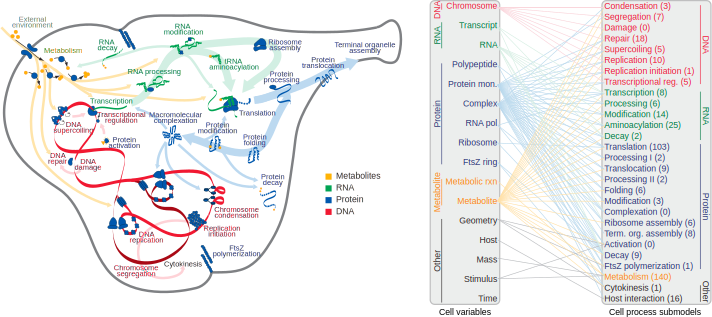
\includegraphics[width=0.95\columnwidth]{fig/cellprocessesdiagram.pdf}
\end{center}
\caption{A schematic depiction of some processes underlying a prokaryotic organism (\emph{M. genitalium}) used in developing an individual life-cycle computational model. Adapted from \cite{Karr2012}.}
\label{fig:cellprocess}
\end{figure}
Many salient features of biological organization at the level of a simple parasitic single-celled organism have recently been encapsulated in a unified computational model of the life-cycle of such a cell. In particular, this model tracks 16 important cell-level variables that each depend on a specified subset of 28 cellular processes. Figure \ref{fig:cellprocess} shows a schematic depicting the interrelationships between these processes specified in the context of this model.

From an energetic, and thus physical, perspective, metabolic processes like the citric acid cycle (see Figure \ref{fig:ctacyc}) are certainly fundamental to the existence and persistence of all evolvable systems. As shown in Figure~\ref{fig:cellprocess}, metabolic processes form the connection between the dual components induced by considering cells as systems in the first place: the internal and the external environment. Moreover, it has been argued that metabolic processes form the basis or atomic level in a hierarchy of cellular processes. From this point of view, the complex regulatory networks involving small molecules, DNA, proteins and other molecular types are viewed as subservient to and layered atop core metabolic processes. Moreover, metabolic processes may be viewed as causally prior to the origin of evolution \cite{Braakman2012,Braakman2012a}.

These facts regarding the fundamental nature of metabolic networks motivate the attempt to model metabolism abstractly in order to characterize and parse its essential properties from those that may represent unnecessary historical contingency. There are several existing formalisms that for constructing dynamical models of metabolic processes. However, these do not attempt to explain how metabolic processes originated or how they are maintained by complex networks of molecular interactions that are not themselves considered only as indirectly related to metabolic processes.

Robert Rosen suggested a formalism for metabolic networks that does attempt to abstractly incorporate the interrelationships between metabolic networks and the other regulatory networks involving interactions among DNA, RNA, and proteins \cite{Rosen1972,Rosen1991}. At the heart of this formalism lies the conceptual conviction that, in some sense, metabolic processes must be able to intrinsically construct at least some of their own causal antecedents. The justification for stating ``at least some of'' as opposed to all is on the basis of taking the distinction between metabolic substrate and enzyme very seriously.

In the context of a network of biochemical reactions, the heuristic distinction between metabolic substrates and enzymes is made on the basis of knowledge about the input and output of any given biochemical reaction. Those inputs that emerge from a biochemical reaction with relatively little to no change in their structure are considered to be enzymes and those whose structure is altered are considered to be substrates whose altered forms are referred to as products.

\begin{figure}
\begin{center}
\noindent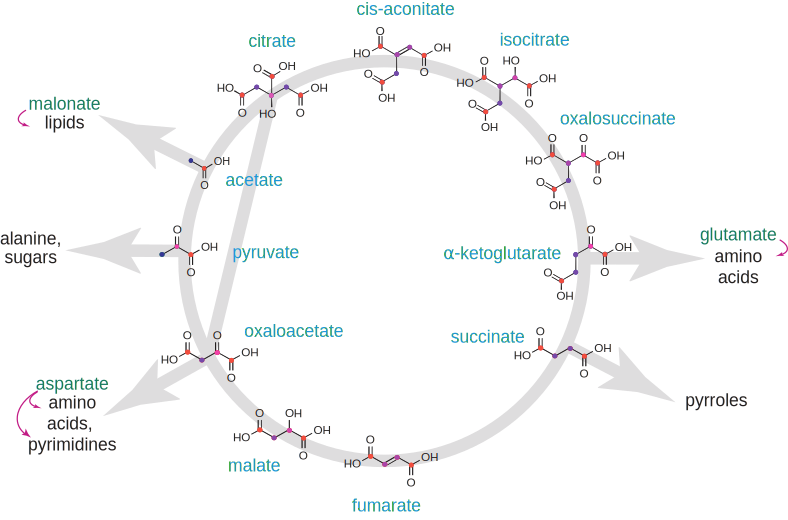
\includegraphics[width=0.7\columnwidth]{fig/rTCA_skeleton.pdf}
\end{center}
\caption{A depiction of the structure of the citric acid cycle and the products of the associated pathways for which it generates substrates.}
\label{fig:ctacyc}
\end{figure}

A situation analogous to the enzyme-substrate-product abstraction \todo{this terminology is used if nowhere else in the main BioPAX publication} is formalized in a fundamental manner in type theory, category theory (see Materials and Methods) and the relationship between them. That a distinction between object and morphism was perhaps conceptually fruitful was originally suggested in Russell and Whitehead's type theory as a means of circumventing the self-referential Russell's (also known as Barber's) paradox of set theory in which one can not determine internal to the language of set theory whether a set of all sets that contain themselves contains itself or not \cite{Bell2012}. In type theory a hierarchy is introduced that is analogous to the distinction fundamental to the definition of a category in category theory (see Materials and Methods) between objects (which are like substrates and products in terms of metabolic networks) and morphisms (which play the role of enzymes). In category theory, this distinction propagates up a hierarchy of higher-order functions where if we are in a category having a terminal, $1$, and exponential objects and we consider two objects $A$ and $B$ and morphisms between them, the collection of which is represented internal to a given category as a so-called exponential object $B^A$ or externally as $Hom(A,B)$ one of which might be $f \colon A \rightarrow B$ then the respective \emph{elements} of $A$, $B$ and $B^A$ are essentially of different types. From this perspective, while it is possible to \emph{evaluate} an element $f:B^A$ read ``an element $f$ of type $B^A$ given by $f \colon 1 \rightarrow B^A$'' at an element $a:A$ given by $a \colon 1 \rightarrow A$ to arrive at some element $b:B$ given by $b \colon 1 \rightarrow B$ it is not possible to likewise \emph{evaluate} an element $a:A$ at another element $a':A$ as this kind of statement is simply not able to be expressed within the confines of the language. If it were possible to do such a thing in some more expressive meta-language of which category theory only represents a fragment, then we can imagine that while reasoning within the language of category theory itself we have restricted ourselves to a state in which we are completely unaware and unable to become aware of this capacity.

The enzyme-substrate-product abstraction can be interpreted in terms of symmetric monoidal categories and depicted using corresponding string diagrams. Any metabolic reaction such as one of the first steps in the tricarboxylic acid cycle depicted in Figure \ref{fig:ctacyc} can be viewed as a morphism acting on tensored objects. The way this metaphor is constructed is to associate to a biochemical reaction such as
$$
\text{Oxaloacetate } + \text{Acetyl CoA} + H_2O \xrightarrow[]{\text{Citrate synthase}} \text{Citrate} + \text{CoA-SH},
$$
abstract labels
$$
s_1 + s_2 + s_3 \xrightarrow[]{m_1} p_1 + p_2.
$$
This can be done for any biochemical reaction and at any level of abstraction. For example we can do the same for the net reaction that occurs for each iteration of the TCA cycle as
$$
\text{Acetyl-CoA} + 3 \text{NAD}^+ + \text{Q} + \text{GDP} + P_i + 3 H_2O \xrightarrow[]{\text{TCA cycle}} \text{CoA-SH} + 3 \text{NADH} + 3H^+ + QH_2 + \text{GTP} + 2 CO_2,
$$
where we now have to abstract from a single enzyme to the composite action of all of the enzymes directly involved in the TCA cycle to which we give the name ``TCA cycle''. The abstract labels that may be associated with this biochemical transformation are
$$
s_1 + s_2 + s_2 + s_2 + s_3 + s_4 + s_5 + s_6 + s_6 + s_6 \xrightarrow[]{f} p_1 + p_2 + p_2 + p_2 + p_3 + p_3  + p_3 + p_4 + p_5 + p_6 + p_6.
$$
The general promiscuity of metabolic interactions in which enzymes recognize a collection of, for the most part very closely, related substrates suggests the representation of these biochemical reactions as tensor products of objects in a category. The intuition behind doing so lies in the fact that if there is a general class of substrates that can substitute for a given one, then instead of specifying a particular one, $s_1$, we should specify an entire set of them $S_1$. Then if there is another set, $S_2$ of substrates that can take the place of $s_2$, and the substrates upon which an enzyme acts is defined on $S_1 \times S_2$, then that enzyme can be said to act on any pair $(s_1,s_2)$ of substrates where $s_1 \in S_1$ and $s_2 \in S_2$. This case of viewing $S_1$ and $S_2$ as sets may come to be seen as being too restrictive in which case we would be forced to consider the abstract tensor product of two objects in a category $S_1 \otimes S_2$, which could then be specialized to a different special case than that in which $S_1$ and $S_2$ are sets. For the simple example of the Citrate synthase catalyzed aldol condensation reaction described above, we arrive at a representation in terms of a morphism in a symmetric monoidal category
\begin{eqnarray*}
m_1 \colon S_1 \otimes S_2 \otimes S_3 &\longrightarrow& P_1 \otimes P_2\\
(s_1,s_2,s_3) &\longmapsto& (p_1,p_2)
\end{eqnarray*}
The adjective ``symmetric'' is appended to monoidal category based upon the assumption that the order of combination of substrates and production of products is unimportant and thus the factors in said tensor products may be permuted. The prototype example of such a monoidal category is the category of sets with cartesian product, but the formalism is not limited to this particular representation. We will proceed thinking in terms of this particular case as a useful mental crutch for grounding intuitions, but its limitations with respect to the capacity to recognize the full generality of the formalism at hand can be severe. Indeed, we will be forced to highlight at least one case where such intuition fails in order to explain the functional closure concept.

\begin{figure}
\begin{center}
\noindent\includegraphics[width=0.9\columnwidth]{fig/blockdiagtop.pdf}
\end{center}
\caption{An abstraction of metabolic networks that can be interpreted in terms of symmetric monoidal categories and their associated string diagrams (see Materials and Methods).}
\label{fig:metabolicstringdiag}
\end{figure}

The metabolic network formalism interpreted in symmetric monoidal categories then applies to the case in which we string together metabolic processes. An example of this is presented in Figure \ref{fig:metabolicstringdiag}. In this diagram, we have the following morphisms:
\begin{eqnarray*}
m_1 \colon S_1 \otimes S_2 &\longrightarrow& P_1 \otimes I_1,\\
m_2 \colon I_1 &\longrightarrow& P_2 \otimes I_2,\\
m_3 \colon I_2 \otimes S_3 &\longrightarrow& P_3 \otimes P_4.
\end{eqnarray*}
These morphisms can be composed as
$$
f \cong (m_1 \circ m_2) \circ m_3 \cong m_1 \circ (m_2 \circ m_3) \cong m_1 \circ m_2 \circ m_3,
$$
where further identifying $A \cong S_1 \otimes S_2 \otimes S_3$ and $B \cong P_1 \otimes P_2 \otimes P_3 \otimes P_4$ allows us to express any metabolic network represented in the form depicted in Figure \ref{fig:metabolicstringdiag} regardless of the more or less complicated nature of intermediate interactions concisely as
$$
\xymatrix@1{
	A\ar[r]^-{f} & B.
	}
$$
In general we can consider any case of $f \colon \prod_i S_i \rightarrow \prod_j P_j$ as being denoted by $f \colon A \rightarrow B$ for $A \cong \prod_i S_i$ and $B \cong \prod_j P_j$. An element $a \colon A$ then represents a tuple $(s_1, s_2, \ldots, s_N)$ that expresses a state of metabolic input substrates and likewise for the metabolic products $b \colon B$ representing $(p_1, p_2, \ldots, p_M)$.

\begin{figure}
\begin{center}
\noindent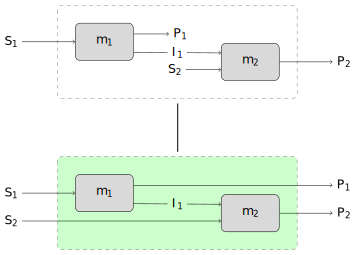
\includegraphics[width=0.5\columnwidth]{fig/blockassoclaw.pdf}
\end{center}
\caption{A demonstration of a simple graph rewrite or reduction rule that can be applied to metabolic processes. This rule can be used in the reduction of a simple model of the citric acid cycle to an effective network.}
\label{fig:stringassoclaw}
\end{figure}

A graph rewrite rule can be derived from the associative composition law that is valid in symmetric monoidal categories in terms of string diagrams like that of Figure~\ref{fig:metabolicstringdiag}. In this case we have template metabolic processes given by
\begin{eqnarray*}
m_1 \colon S_1 &\longrightarrow& P_1 \otimes I_1,\\
m_2 \colon I_1 \otimes S_2 &\longrightarrow& P_2,
\end{eqnarray*}
shown in the top panel of Figure \ref{fig:stringassoclaw}. Following the application of the rewrite rule presented in Figure \ref{fig:stringassoclaw} we have the composite effective metabolic process
\begin{eqnarray*}
m_{1}m_{2} \equiv m_1 \circ m_2 \colon S_1 \otimes S_2 &\longrightarrow& P_1 \otimes P_2,
\end{eqnarray*}
where we note that the intermediate $I_1$ has been eliminated from both the inputs and outputs of the $m_1$ and $m_2$ processes.

This formalism has been previously applied, albeit not in the explicit context of symmetric monoidal categories, to reduce via associative composition the citric acid cycle to a smaller collection of effective reactions. The steps involved in this process are depicted in Figure \ref{fig:ctacycred}. The fully reduced form of the citric acid cycle presented in Figure \ref{fig:ctacycred}d will be used in what proceeds to provide a biological example with respect to which the additional molecular interactions that may be necessary in order to achieve functional closure may be defined.

\begin{figure}
\begin{center}
\noindent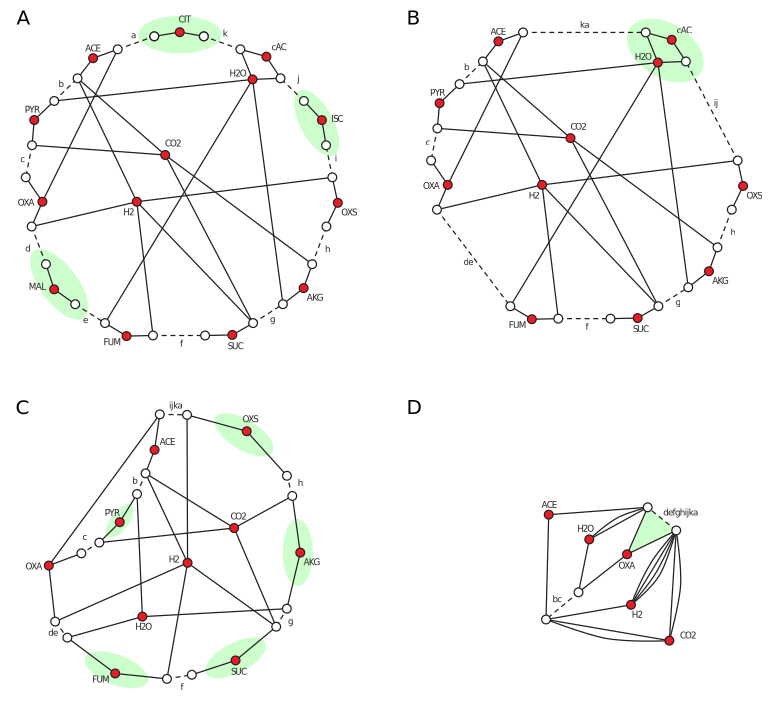
\includegraphics[width=0.9\columnwidth]{fig/rTCA-reduction.pdf}
\end{center}
\caption{A demonstration of the reduction of the biochemical reactions comprising the citric acid cycle according to the graph rewrite rule depicted in Figure \ref{fig:stringassoclaw}. This figure is adapted from the citric acid cycle reduction process developed in \cite{Braakman2012a}}
\label{fig:ctacycred}
\end{figure}


\section*{Functional closure}
\subsection*{Functional closure as an invariant property of evolvable systems}

In this section, we will attempt to explain the functional closure property in category theoretic terms. The abstract components have been related to biological ones in the previous section. The biological property from which Rosen derived his diagram expressing the functional closure concept is metabolism regarded in the manner described above and as depicted in Figure \ref{fig:metabolicstringdiag}. A metabolic mapping in an evolvable system $\mathcal{E}$ can be thought of as a morphism between two objects in $\mathcal{E}$, the latter now regarded as an abstract algebraic category:
\begin{align*}
f \colon A &\longrightarrow B\\
a &\longmapsto f(a)=b
\end{align*}

In category theory, we can imagine the abstract objects and morphisms as specializing to a particular type of algebraic structure and, thus, as a first approximation we can think of both objects as (cartesian product) sets, where $A$ represents a configuration of input substrates and $B$ likewise for metabolite products of metabolic transformations such as $f$. This abstraction of some aspects of an evolvable system could be further developed by substituting more highly structured objects than sets that meet intuitive and otherwise empirically suggested features of evolvable systems. We can consider all such \emph{metabolisms} together as the set of all the different morphisms between these objects referred to, if such an object exists at all, as the \emph{internal} exponential object $B^A$ \footnote{see Materials and Methods for the precise definition of exponetial object} or the \emph{external} hom-set $Mor_{\mathcal{E}}(A,B)$.

The apparently finite nature of evolvable systems, imposes several constraints regarding the maintenance of sufficient concentrations of the components that constitute it. As enzymes necessary for metabolism decay, they must be regenerated, from the metabolic products, or the system comprised of them will disintegrate. In addition, fluctuations in the substrates $A$ have to be corrected by the differential availability and performance of the overall metabolic morphism $f$. Hence, there must be a collection of morphisms from $B$ to $B^A$, one of which can be identified with the information required to \emph{regenerate} the enzymes necessary for core metabolic processes:
\begin{align*}
g \colon B &\longrightarrow B^A\\
b &\longmapsto g(b)=f
\end{align*}
This \emph{regeneration} system itself represented by $g \in B^{A^B}$ is also assumed to have a finite lifetime and thus requires a form of \emph{meta-regeneration} by some other system:
\begin{align*}
h \colon B^A & \longrightarrow B^{A^B}\\
f & \longmapsto h(f)=g.
\end{align*}	
In the biological metaphor commonly associated to this abstract construction, this \emph{meta-regeneration} system is associated either to the maintenance of some degree of structural invariance in the topology of the combined gene regulatory and metabolic interaction networks underlying an organism. In this light, this process may be associated to the DNA replication and reproduction process. In any case, the argument proliferating hierarchical levels of organization necessary to strive toward functional closure may be continued \emph{ad infinitum} (i.e. the next step would be to ask for the origin of $h$ and to posit the existence of another higher-order morphism that takes $g$ as input and produces $h$, see Figure \ref{fig:hom}b). 

From a biological perspective, systems of the form described may be able to avoid such an infinite regress by achieving a form of \emph{functional closure} in which, for example, we can materially identify a metabolic product $B$ with a replication function $h$ or perhaps even with the entire set of replication functions $B^{A^B{^B{^A}}}$. If we take the former case then we have introduced a problem that cannot be dealt with given the definition of a category because of the fundamental typing distinction therein between objects and morphisms. Although we might be able to associate an element or point of the object or type $B$ with $h \in B^{A^B{^B{^A}}}$, we sustain a typing error if we attempt to express the fact that these are materially equivalent because $h \colon 1 \rightarrow B$ is of type $B$ while $h \colon B^A \rightarrow B^{A^B}$ is of type $B^{A^B{^B{^A}}}$. Thus we would attempt to state $h:B = h:B^{A^B{^B{^A}}}$, but this is impossible to do, at least naively, within category theory as it produces a type error due to the fact that equations are only allowed between elements (respectively paths) with the same type (respectively with the same domain and codomain) Figure \ref{fig:hom}a. The other option is to avoid attempting to identify such elements and attempt to simply identify objects themselves. In this sense, we would attempt to express closure internally as $B \cong B^{A^B{^B{^A}}}$ or externally as $Mor_{\mathcal{E}}(1,B) \cong Mor_{\mathcal{E}}(B^A,B^{A^B})$. This approach could be considered to solve the typing issue since we could more explicitly state that $B \colon Set \cong B^{A^B{^B{^A}}} \colon Set$ or more generally for any category $B \colon Ob(\mathcal{E}) \cong B^{A^B{^B{^A}}} \colon Ob(\mathcal{E})$. However, we have now implied something stronger and less intuitive about the biological meaning of functional closure by stating that the set of metabolites is somehow isomorphic to the set of \emph{all possible} replication morphisms. Moreover, if such a relationship were to be satisfied, it could only be satisfied by the most trivial case in the category of sets $A = \{*\} = B$ so that $|B|=1=|B^{A^B{^B{^A}}}|$.

We have not yet attempted to make explicit how it might be possible to perform the identification between an element of type $B$ and another of type $B^{A^B{^B{^A}}}$ as expressed in Figure \ref{fig:hom}c. The original argument describing functional closure in a sense settles for stating something weaker than what we have already suggested is impossible to do directly within category theory (i.e. to state for some $h$, $h:B = h:B^{A^B{^B{^A}}}$). The most important feature of this argument is the concept of an evaluation map (see Materials and Methods) or morphism, which is intrinsic to the definition of exponential objects and thus evaluation maps exist in categories, like the primary example of the category of $\mathbf{Sets}$ we have considered thus far, having exponential objects. Given a category with products and exponentials, the evaluation map can be curried (i.e. in this case a function of two variables that returns a value can be converted to a function of one variable that returns a function) in the following manner
\begin{prooftree}
				\AxiomC{$B^{A} \times A \xrightarrow[]{ev} B$}
				\UnaryInfC{$A \xrightarrow[]{\hat{ev}} B^{B^A}$}
\end{prooftree}
where the maps $\hat{ev}$ are defined pointwise as
\begin{align*}
\hat{ev}(a) \equiv ev_a \colon B^A &\longrightarrow B,\\
f &\longmapsto ev(f,a) = f(a).
\end{align*}
This construction can be applied analogously at the next level regarding the evaluation of functions of the type $B^{A^B}$, by applying them to arguments of type $B$, to functions of the type $B^A$. The currying of the evaluation map is given by
\begin{prooftree}
				\AxiomC{$B^{A^B} \times B \xrightarrow[]{ev} B^A$}
				\UnaryInfC{$B \xrightarrow[]{\hat{ev}} B^{A^{B^{A^B}}}$}
\end{prooftree}
where the maps $\hat{ev}$ are defined pointwise as
\begin{align*}
\hat{ev}(b) \equiv ev_b \colon B^{A^B} &\longrightarrow B^A,\\
g &\longmapsto ev(g,b) = g(b).
\end{align*}
Although the continuation of the functional closure argument may also be applied in the first case of $ev_a$, we will apply it to the next level involving $ev_b$ to maintain the intuitive property that the metabolic substrate configuration represented by $A$ also represents material being extracted from the environment while functional closure is assumed to be achieved internal to the metabolic network (represented by $f$) and the regulatory apparatus (represented by $g$ and $h$) layered on top of it despite the material connection via $A$ to the environment.

We first consider the preimages of the evaluation morphisms as
\begin{align*}
\hat{ev}^{*}(b) \equiv ev^{*}_b \colon B^A &\longrightarrow B^{A^B},\\
f &\longmapsto g |g(b)=f.
\end{align*}
If, in this case, the evaluation morphism can be shown to have an inverse (i.e. $\hat{ev}^{*} \circ \hat{ev} = 1_A$ and $\hat{ev} \circ \hat{ev}^{*}= 1_{B^{B^A}}$) for some potentially restricted domain of definition of $\hat{ev}$ then the inverse morphism can also be defined pointwise as 
\begin{align*}
\hat{ev}^{-1}(b) \equiv ev^{-1}_b \colon B^A &\longrightarrow B^{A^B},\\
f &\longmapsto g | g(b) = f.
\end{align*}
In this sense, if there is a unique $g$ satisfying $g(b)=f$ for each combination of $b$ and $f$ in the restricted domains of definition then $b$ and $f$ can be viewed as determining $g$. This relieves what otherwise appears to be the necessity of positing the existence of an $h$ to answer the question of the origin of $g$. This is the weaker statement that is supported by this argument as compared to the stronger version, which could ostensibly be expressed as $b:B = h:B^{A^{B^{B^A}}}$.

\begin{figure}
\begin{center}
\noindent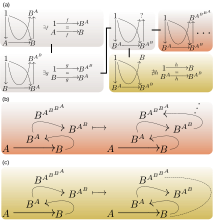
\includegraphics[width=0.75\columnwidth]{fig/mrcatclosure.pdf}
%\noindent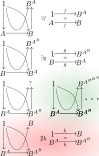
\includegraphics[width=0.24\columnwidth]{fig/mrcatprob.pdf}
\end{center}
\caption{Rosen's diagram attempting a depiction of functional closure in a cartesian closed category. (a) The top-left panel shows the identification of morphisms with domain $A$ and codomain $B$ with elements of the exponential object $B^A$. The bottom-left panel shows the analogous relationship between morphisms with domain $B$ and codomain $B^A$ and the exponential object $B^{A^B}$. On the right, two alternatives are shown in the last step. Either one can (b) continue on the path leading to infinite regress or (c) take the path leading to immediate closure.}
\label{fig:hom}
\end{figure}

\subsection*{Functional closure expressed in a type-free setting}
This argument describing functional closure so far suggests constraints by which we may be able to \emph{determine} some $h$ via $b$ (and also $f$), but so long as the ultimate goal is to state that for some $b$, $b:B = h:B^{A^B{^B{^A}}}$, it appears that it cannot be done in an obvious way in category theoretic terms. This is a result of the typing discipline inherent to the category theoretic description used thus far. We will ultimately find that we can re-express a stronger form of the functional closure in category theoretic terms, but in a manner that it is not obvious how to define directly within category theory. We thus first re-consider the expression of functional closure in terms of another language, the lambda calculus, which has both type-free and varying degrees of typed forms \cite{Barendregt1985} before returning to the so-called categorical semantics that enable the re-expression of this stronger form of functional closure in category theoretic terms.

If we reconsider the discussion in the previous section without regard for any typing discipline, we can summarize the proliferation of levels of organization up through the first three discussed in the following system of equations
\begin{align*}
f(a)&=b,\\
g(b)&=f,\\
h(f)&=g.
\end{align*}
It is trivial to express the functional closure property so long as we are able to disregard any typing discipline by identifying $h$ with $b$. In this case we can express functional closure as
\begin{align*}
f(a)&=b,\\
g(b)&=f,\\
b(f)&=g.
\end{align*}

%In order for  $\mathcal{E}$ to be functionally closed every morphism must be represented by or be in turn an object of the category. As we have stated, the set of functions $Mor_{\mathcal{E}}(A,B)$ between two objects in the category can be represented by the exponential object $B^A$. These exponential objects are associated with so-called evaluation maps both for the metabolic morphisms:
%\begin{align*}
%e_f : B^A \times A &\longrightarrow B,\\
%(f,a) & \longmapsto f(a),
%\end{align*}
%and for the maintenance system:
%\begin{align*}
%			e_g: B^{A^B} \times B &\longrightarrow B^A,\\
%	    			            (g,b) & \longmapsto    g(b).
%\end{align*}		
%We can take the system as described and develop all the exponentiations of its maps and represent all the evaluation functions of its exponential objects:		
%$$
%			\xymatrix{
%			 ... & ... & ... \\
%			  B^{A^{B^A}} \times A \ar[r]_-{\epsilon} \ar[u]^-{..^A} & B^{A^B} \ar[u]^-{..} & B^{A^{B^B}} \times B\ar[l]^-{\epsilon}\ar[u]^-{..^B} \\
%			 B^{A^A} \times A \ar[r]_-{\epsilon} \ar[u]^-{r^A} & B^A \ar[u]^-{r} & B^{A^B} \times B\ar[l]^-{\epsilon}\ar[u]^-{r^B} \\
%			B^A \times A \ar[r]_-{\epsilon} \ar[u]^-{g^A} & B \ar[u]^-{g} & B^B \times B\ar[l]^-{\epsilon}\ar[u]^-{g^B} \\
%			A^A \times A \ar[r]_-{\epsilon} \ar[u]^-{f^A} & 
%			A\ar[u]^-{f} & A^B\times B\ar[l]^-{\epsilon}\ar[u]^-{f^B} }
%$$
%
%Once the second level of exponentiation is reached, the system is in some sense already closed, and the higher level exponential objects can be reduced to lower level morphisms. This is explained in terms of the $\times \dashv Hom$ adjunction (see the appendix). 
%\begin{align*}
%- \times A: \mathcal{E} & \rightleftarrows \mathcal{E}: (-)^A
%\end{align*}
%For any $B \in Obj(\mathcal{E})$ there is a bijection:
%\begin{align*}
%\Mor_{\mathcal{E}}(B \times A, B) & \cong  \Mor_{\mathcal{E}}(B, B^A)
%\end{align*}
%$$
%	\frac{B \times A \longrightarrow B}{B \longrightarrow B^A}
%$$
%For the case of $B$ we obtain the \emph{maintenance} map as the exponential transpose $g \colon B \rightarrow B^A$ of $\bar{g}:B \times A \rightarrow B$
%$$
%	\xymatrix{
%	& B \times A \ar[d]^{g \times 1_A} \ar[dl]_{\bar{g}} & B \ar@{.>}[d]^{g}\\
%	B & B^A \times A \ar[l]^{\epsilon_B} & B^A}
%$$
%where the counit of the $\times \dashv Hom$ adjunction is the evaluation map
%$$
%	\epsilon_B = ev_B \colon B^A \times A \longrightarrow B.
%$$
%In the analogous way, we have an adjunction involving $B^A$
%\begin{align*}
%\Mor_{\mathcal{E}}(B^A \times A, B) & \cong  \Mor_{\mathcal{E}}(B^A, B^{A})
%\end{align*}
%$$
%	\frac{B^A \times A \longrightarrow B}{B^A \longrightarrow B^{A}}
%$$
%$$
%	\xymatrix{
%	& B^A \times A \ar[d]^{1_{B^A} \times 1_A} \ar[dl]_{\overline{1_{B^A}}} & 	B^A \ar@{.>}[d]^{1_{B^A}}\\
%	B & B^A \times A \ar[l]^-{\overline{1_{B^A}}} & B^A}
%$$
%If we repeat the process exponentiating $B^A$ by $B$, the \emph{replication} map is obtained:	
%\begin{align*}
%- \times B: \mathcal{C} & \rightleftarrows \mathcal{C}: (-)^B\\
%\Mor_{\mathcal{C}}(B^A \times B, B^A) & \cong  \Mor_{\mathcal{C}}(B^A, B^{A^B})
%\end{align*}
%$$
%			\frac{B^A \times B \longrightarrow B^A}{B^A \longrightarrow B^{A^B}}
%$$
%$$ 
%	\xymatrix{
%	& B^A \times B \ar[d]^-{h \times 1_B} \ar[dl]_{\bar{h}} & B^A \ar@{.>}[d]^-{h}\\
%	B^A & B^{A^B} \times B \ar[l]^{\epsilon_{B^A}} & B^{A^B}}
%$$
%Continuing this process with $B^{A^B}$
%\begin{align*}
%- \times B: \mathcal{C} & \rightleftarrows \mathcal{C}: (-)^B\\
%\Mor_{\mathcal{C}}(B^{A^B} \times B, B^A) & \cong  \Mor_{\mathcal{C}}(B^{A^B}, B^{A^B})
%\end{align*}
%$$
%	\frac{B^{A^B} \times B \longrightarrow B^A}{B^{A^B} \longrightarrow B^{A^B}}
%$$
%$$
%	\xymatrix{
%	& B^{A^B} \times B \ar[d]^{1_{B^{A^B}} \times 1_B} 	\ar[dl]_{\overline{1_{B^{A^B}}}} & B^{A^B} \ar@{.>}[d]^{1_{B^{A^B}}}\\
%	B^A & B^{A^B} \times B \ar[l]^-{\overline{1_{B^{A^B}}}} & B^{A^B}}
%$$
%To summarize, we can attempt to express functional closure at the first level by the following series of deductions
%\begin{prooftree}
%	\AxiomC{$B^A \times A \longrightarrow B$}
%	\UnaryInfC{$B^A \longrightarrow B^A$}
%	\UnaryInfC{$1 \longrightarrow B^A \longrightarrow B^A$}							\UnaryInfC{$1 \times A \longrightarrow B \longrightarrow B^A$}
%	\UnaryInfC{$A \longrightarrow B \longrightarrow B^A$}
%	\UnaryInfC{$A \longrightarrow B^A$}
%\end{prooftree}
%If we prefer to continue with the biological metaphor initiated by Rosen's diagram, we can identify the functional closure property at the second level		
%\begin{prooftree}
%				\AxiomC{$B^{A^B} \times B \longrightarrow B^A$}
%				\UnaryInfC{$B^{A^B} \longrightarrow B^{A^B}$}
%				\UnaryInfC{$1 \longrightarrow B^{A^B} \longrightarrow B^{A^B}$}
%				\UnaryInfC{$1 \times B \longrightarrow B^A \longrightarrow B^{A^B}$}
%				\UnaryInfC{$B \longrightarrow B^A \longrightarrow B^{A^B}$}
%				\UnaryInfC{$B \longrightarrow B^{A^B}$}
%\end{prooftree}
%Closing the system by:
%\begin{align*}
%- \times B: \mathcal{E} & \rightleftarrows \mathcal{E}: (-)^B\\
%\Mor_{\mathcal{E}}(B^{A^B} \times B, B^{A^B}) & \cong  \Mor_{\mathcal{E}}(B^{A^B}, B^{A^{B^B}})
%\end{align*}
%
%			$$
%			\xymatrix{
%			& B^{A^B} \times B \ar[d]^-{i \times 1_B} \ar[dl]_{\bar{i}} & B^{A^B} \ar@{.>}[d]^-{i}\\
%			B^{A^B} & B^{A^{B^B}} \times B \ar[l]^{\epsilon} & B^{A^{B^B}}
%			}
%			$$
%		$$
%			\frac{B^{A^B} \times B \longrightarrow B^{A^B}}{B^{A^B} \longrightarrow B^{A^{B^B}}}
%		$$
%		the counit is the evaluation map
%		$$
%			\epsilon = ev_{B^{A^B}} \colon B^{A^{B^B}} \times B \longrightarrow B^{A^B}
%		$$
%	

\section*{Discussion}

% You may title this section "Methods" or "Models". 
% "Models" is not a valid title for PLoS ONE authors. However, PLoS ONE
% authors may use "Analysis" 
\section*{Materials and Methods}
\subsection*{Categories\todo{so far, this section is lifted from planetmath.org.}}
%!TEX root = ../notes.tex
An intuitive picture to which one can anchor intuition when thinking in category theoretic terms is presented in \ref{fig:intextdiag}. In category theory, one can always consider the duality between the intrinsic structure of \emph{objects} and the manner in which that intrinsic structure can be expressed externally in terms of patterns of constraints placed upon the relationships between \emph{morphisms} among objects.

\begin{figure}
\begin{center}
\noindent
\includegraphics[width=0.8\columnwidth]{fig/intextdiag.pdf}
\end{center}
\caption{In the external diagram on the left one simply considers \emph{objects} such as $A$,$B$, and $C$ and morphisms between them $f$, $g$, and $m$. The internal perspective, which in this case is specific to the category of $\mathbf{Sets}$, demonstrates the particular manner in which the equation $g \circ f = m$ may be satisfied in terms of the internal structure of the objects $A$, $B$, and $C$. Of course, in this case there are many other ways of satisfying the given equation; however, there are also questions that can be answered about the relationship between $A$, $B$, and $C$ given either $g \circ f = m$ or $g \circ f \neq m$ without necessarily knowing the particular manner in which either equation is satisfied by the relationships among the internal structures of the objects involved.}
\label{fig:intextdiag}
\end{figure}

%\input{tex/category.tex}
%
%\subsection*{Cartesian closed category}
%A category $\mathcal{C}$ with finite products is said to be \emph{Cartesian closed} if each of the following functors has a right adjoint
\begin{enumerate}
\item $\textbf{0}:\mathcal{C}\to \textbf{1}$, where $\textbf{1}$ is the trivial category with one object $0$, and $\textbf{0}(A)=0$
\item the diagonal functor $\delta: \mathcal{C}\to \mathcal{C}\times\mathcal{C}$, where $\delta(A)=(A,A)$, and
\item for any object $B$, the functor $(-\times B):\mathcal{C}\to\mathcal{C}$, where $(-\times B)(A)=A\times B$, the product of $A$ and $B$.
\end{enumerate}
Furthermore, we require that the corresponding right adjoints for these functors to be
\begin{enumerate}
\item any functor $\textbf{1}\to\mathcal{C}$, where $0$ is mapped to an object $T$ in $\mathcal{C}$.  $T$ is necessarily a terminal object of $\mathcal{C}$.  
\item the product (bifunctor) $(-\times -): \mathcal{C} \times \mathcal{C}\to \mathcal{C}$ given by $(-\times -)(A,B)\mapsto A\times B$, the product of $A$ and $B$.
\item for any object $B$, the exponential functor $(-^B):\mathcal{C}\to\mathcal{C}$ given by $(-^B)(A)=A^B$, the exponential object from $B$ to $A$.
\end{enumerate}

In other words, a Cartesian closed category $\mathcal{C}$ is a category with finite products, has a terminal objects, and has exponentials.  It can be shown that a Cartesian closed category is the same as a finitely complete category having exponentials.

Examples of Cartesian closed categories are the category of sets \textbf{Set} ( terminal object: any singleton; product: any Cartesian product of a finite number of sets; exponential object: the set of functions from one set to another)  the category of small categories \textbf{Cat} (terminal object: any trivial category; product object: any finite product of categores; exponential object: any functor category), and every elementary topos.
%
%\subsection*{Monoidal categories}
%A \emph{monoidal category} is a category which has the structure of a monoid, that is, among the objects there is a binary operation which is associative and has an unique neutral or unit element.   Specifically, a category $\mathcal{C}$ is \emph{monoidal} if
\begin{enumerate}
\item there is a bifunctor $\otimes: \mathcal{C}\times\mathcal{C}\to \mathcal{C}$, where the images of object $(A,B)$ and morphism $(f,g)$ are written $A\otimes B$ and $f\otimes g$ respectively,
\item there is an isomorphism $a_{ABC}: (A\otimes B)\otimes C \cong A\otimes (B\otimes C)$, for arbitrary objects $A,B,C$ in $\mathcal{C}$, such that $a_{ABC}$ is natural in $A,B$ and $C$.  In other words,
\begin{itemize}
\item $a_{-BC}: (-\otimes B)\otimes C \Rightarrow -\otimes(B\otimes C)$ is a natural transformation for arbitrary objects $B,C$ in $\mathcal{C}$,
\item $a_{A-C}: (A\otimes -)\otimes C \Rightarrow A\otimes(-\otimes C)$ is a natural transformation for arbitrary objects $A,C$ in $\mathcal{C}$,
\item $a_{AB-}: (A\otimes B)\otimes - \Rightarrow A\otimes(B\otimes -)$ is a natural transformation for arbitrary objects $A,B$ in $\mathcal{C}$,
\end{itemize}
\item there is an object $I$ in $\mathcal{C}$ called the \emph{unit object} (or simply the \emph{unit}),
\item for any object $A$ in $\mathcal{C}$, there are isomorphisms: 
$$l_A: I\otimes A\cong A \qquad \mbox{and} \qquad r_A: A\otimes I\cong A,$$
such that $l_A$ and $r_A$ are natural in $A$: both $l: I\otimes - \Rightarrow -$ and $r: -\otimes I\Rightarrow - $ are natural transformations
\end{enumerate}
satisfying the following commutative diagrams:
\begin{itemize}
\item \emph{unit coherence law}
$$\xymatrix@+=2cm{(A\otimes I)\otimes B \ar[rr]^{a_{AIB}} \ar[dr]_{r_A\otimes 1_B} & & A\otimes (I\otimes B) \ar[dl]^{1_A \otimes r_B} \\ & A\otimes B & }$$
\item \emph{associativity coherence law}
$$\xymatrix@+=2cm{((A\otimes B)\otimes C)\otimes D \ar[rr]^{a_{A\otimes B,C,C}} \ar[d]_{a_{ABC}\otimes 1_D} &&  (A\otimes B)\otimes (C\otimes D) \ar[dd]^{a_{A,B,C\otimes D}} \\ 
(A\otimes (B\otimes C))\otimes D \ar[d]_{a_{A,B\otimes C,D}} && \\
A\otimes ((B\otimes C)\otimes D) \ar[rr]_{1_A\otimes a_{BCD}} && A \otimes (B\otimes (C\otimes D))}$$
\end{itemize}
The bifunctor $\otimes$ is called the \emph{tensor product} on $\mathcal{C}$, and the natural isomorphisms $a,l,r$ are called the \emph{associativity isomorphism}, the \emph{left unit isomorphism}, and the \emph{right unit isomorphism} respectively.

Some examples of monoidal categories are
\begin{itemize}
\item
A prototype is the category of isomorphism classes of vector spaces over a field $\mathbb{K}$, herein the tensor product is the associative operation and the field $\mathbb{K}$ itself is the unit element.
\item
The category of sets is monoidal.  The tensor product here is just the set-theoretic cartesian product, and any singleton can be used as the unit object.
\item
The category of (left) modules over a ring $R$ is monoidal.  The tensor product is the usual tensor product of modules, and $R$ itself is the unit object.
\item
The category of bimodules over a ring $R$ is monoidal.  The tensor product and the unit object are the same as in the previous example.
\end{itemize}
%
%\subsection*{Symmetric monoidal categories}
%\input{tex/symmetricmonoidalcategory.tex}

% Do NOT remove this, even if you are not including acknowledgments
\section*{Acknowledgments}


%\section*{References}
\bibliographystyle{plos2009}
% The bibtex filename
\bibliography{bib/books,bib/papers}

\section*{Figure Legends}

\section*{Tables}

\end{document}

